% !TEX root = ../thesis.tex

\chapter{Hintergrund}
\label{background}

Zum besseren Verständnis der weiteren Verlaufs dieser Arbeit, dient dieses Kapitel zur Einführung in die zugrundeliegenden Themen. Dazu wird zunächst die featurebasierte Softwareentwicklung erläutert, ehe dann der Themenbereich des Machine Learnings vorgestellt wird. Dazu werden die Klassifikation und die Fehlervorhersage mittels Machine Learning erläutert. Unterstützt werden die Abschnitte von Grafiken zum besseren Verständnis der Zusammenhänge.
\\
\hrule

\section{Featurebasierte Softwareentwicklung}
\label{feat-develop}

Das zentrale Konzept hinter der featurebasierten Softwareentwicklung stellen sogenannte Soft-ware-Produktlinien dar. Wie bereits in der Einleitung erwähnt wurde, beschreiben Software-Produktlinien eine Menge von ähnlichen Softwareprodukten, welche eine gemeinsame Menge von Features sowie eine gemeinsame Codebasis besitzen und sich durch die Auswahl der verwendeten Features unterscheiden, sodass eine breite Variabilität innerhalb einer Produktlinie entstehen kann \cite{Apel2013,Thuem2014}.

Der zentrale Prozess der Generierung einer Software-Produktlinie ist in \autoref{fig:spl} dargestellt. Aufgeteilt wird dieser Prozess in das Domain Engineering und das Application Engineering. Im Rahmen des Domain Engineerings wird ein sogenanntes Variabilitätsmodell (Variability Model) erstellt, welches die wählbaren Features und Constraints für mögliche Selektionen beschreibt \cite{Apel2013}. Gängige Implementationstechniken für Features reichen von einfachen Lösungen durch Annotationen basierend auf Laufzeitparametern oder Präprozessor-Anweisungen bis hin zu verfeinerten Lösungen basierend auf erweiterten Programmiermethoden, wie zum Beispiel Aspektorientierung. In einigen dieser Implementierungstechniken wird jedes Feature wird als wiederverwendbares Domain Artifact modelliert und gekapselt, welches im Prozess des Application Engineerings in Form einer Konfiguration zusammen mit weiteren Features, im Hinblick auf die gewünschte Funktionalität der Software, ausgewählt werden kann. Ein Software Generator erzeugt dann die gewünschten Softwareprodukte basierend auf den bereits zuvor genannten Implementationstechniken für Features.

\begin{figure}[H]
    \centering
    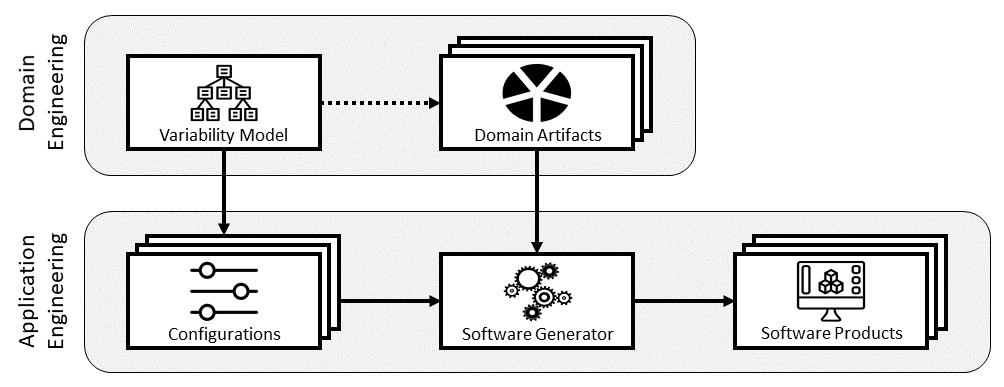
\includegraphics[width=\textwidth]{images/SPL}
    \caption{Generierung von Software-Produktlinien nach \cite{Thuem2014}\label{fig:spl}}
\end{figure}

Die in dieser Arbeit betrachtete Implementierungstechnik von Features basiert auf Anweisungen beziehungsweise Bedingungsdirektiven des C-Präprozessors. Die für diese Arbeit relevanten Direktiven lauten \texttt{\#IFDEF} und \texttt{\#IFNDEF}. Einfache Beispieleinsätze für beide Direktiven sind in \autoref{example1} zu sehen, im Kontext der Beispielmethode \texttt{example()}. Die Direktive \texttt{\#IFDEF} leitet den Code des Features \texttt{feature1} ein, welcher mit der Anweisung \texttt{\#ENDIF} endet. Der mit \texttt{//Code feature1} angegebene Codeteil wird genau dann nur ausgeführt, wenn das Feature \texttt{feature1} im Rahmen der Konfiguration des Softwareproduktes definiert beziehungsweise aktiviert ist \cite{Stallmann2016}. In diesem Fall wird die Bedingung der Direktive erfolgreich erfüllt \cite{Stallmann2016}. Sie schlägt fehl, wenn das Feature nicht definiert beziehungsweise aktiviert ist \cite{Stallmann2016}. Die Direktive \texttt{\#IFNDEF} wird für Code verwendet, der ausgeführt werden soll, wenn ein Feature nicht definiert ist. Im Falle des Beispiels wird der in Zeile 7 angedeutete Code nur ausgeführt, wenn \texttt{feature2} nicht aktiviert wurde.
Es besteht zudem die Möglichkeit, Features bzw. ihren Code zu verschachteln. Ein Beispiel dafür ist in \autoref{example2} angegeben. Es ist zu erkennen, dass sich der Code von \texttt{feature2} innerhalb der bedingten Gruppe von \texttt{feature1} befindet. Der in Zeile 5 angedeutete Code kann somit nur ausgeführt werden, wenn \texttt{feature1} aktiviert ist. Im Fall von Verschachtelung beendet ein \texttt{\#ENDIF} immer das nächstgelegene \texttt{\#IFDEF} oder \texttt{\#IFNDEF} \cite{Stallmann2016}. Es besteht zudem die Möglichkeit, Direktiven mittels \glqq und\grqq{} (\texttt{\&\&}, \texttt{and}) oder \glqq oder\grqq{} (\texttt{||}, \texttt{or}) zu erweiterten Bedingungen zu verknüpfen \cite{Stallmann2016}.

\noindent\begin{minipage}{.45\textwidth}
\begin{lstlisting}[caption=Beispieleinsätze von \texttt{\#IFDEF} \\ und \texttt{\#IFNDEF},frame=tlrb,language=C, label=example1]{example1}
void example(){
#IFDEF feature1
	// Code feature1
#ENDIF
// Code
#IFNDEF feature2
	// Code
#ENDIF
// Code
}
\end{lstlisting}
\end{minipage}\hfill
\begin{minipage}{.45\textwidth}
\begin{lstlisting}[caption=Beispiel eines verschachtelten \\ Einsatzes von \texttt{\#IFDEF},frame=tlrb,language=C, label=example2]{example2}
void example(){
#IFDEF feature1
	// Code feature1
	#IFDEF feature2
			// Code feature1 & feature2
	#ENDIF // Ende Code feature2
	// Code feature1
#ENDIF // Ende Code feature1
// Code
}
\end{lstlisting}
\end{minipage}

Die in \autoref{example1} und \autoref{example2} gezeigten Beispiele zeigen jeweils nur den Featurecode in einer Methode beziehungsweise in einer Datei. Fragmente des Featurecodes erstrecken sich jedoch nicht nur möglicherweise mehrfach über eine Datei sondern über mehrere Dateien - der Featurecode ist somit verstreut (englisch: code scattering), um eine Funktionalität des Features in der Gesamtheit der Software zu ermöglichen. Ein Defekt innerhalb eines Fragmentes des Featurecodes kann allerdings dazu führen, dass die gesamte Funktionalität des Features beeinträchtigt oder unterbunden wird, da der Fehler übergreifend wirkt (englisch: cross-cutting). Grafisch dargestellt ist dies in \autoref{fig:cross-cutting}. Dort wirkt sich der Defekt eines Fragments von Feature 3 in einer Datei auf alle weiteren Dateien aus, sodass die Funktionalität des Features beeinträchtigt wird.

\begin{figure}[H]
    \centering
    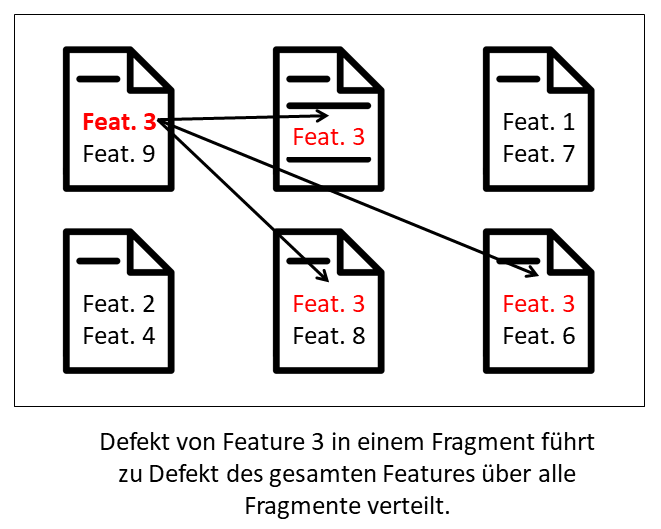
\includegraphics[width=0.6\textwidth]{images/Crosscutting}
    \caption{Auswirkungen eines Defekts in einem Fragment eines Features\label{fig:cross-cutting}}
\end{figure}

\section{Machine-Learning-Klassifikation}
\label{classification}

Das Themengebiet des Machine Learnings (ML) ist in zwei Teilgebiete unterteilt - das unüberwachte ML (englisch: unsupervised ML) und das überwachte ML (englisch: supervised ML). Die Methoden in diesen Teilgebieten verfolgen unterschiedliche Ziele. Im Rahmen des unüberwachten ML werden Prozesse durchgeführt, welche dazu dienen, die Struktur einer unbekannten Eingabemenge an Daten zu erlernen und anschließend zu repräsentieren \cite{Sammut2017}. Eine gängige Anwendung des unüberwachten ML ist das Clustering. Das überwachte ML beschreibt wiederum einen Prozess, welcher beabsichtigt, Vorhersagen über unbekannte Eingabedaten auf Basis der Erlernung einer Abbildungsfunktion zu treffen \cite{Sammut2017}. Die Attribute \glqq unüberwacht\grqq{} und \glqq überwacht\grqq{} erhalten die Methoden aufgrund ihrer Art des Lernens. In der Anwendung des unüberwachten ML werden die Eingabedaten erfasst, gegebenenfalls vorverarbeitet, um dann auf deren Basis ein Modell zu erlernen, welches die Darstellung beziehungsweise Repräsentation der Eingabedaten bestimmt \cite{Alpaydin2010}. Auf der anderen Seite, wird unter Anwendung des überwachten ML, ein Modell auf Basis eines sogenannten \glqq gelabelten\grqq{} (beschrifteten) Datensatzes durch Merkmalsextraktion in Form von Attributen und Lernen auf der Grundlage der extrahierten Merkmale erstellt \cite{Alpaydin2010}. Der Datensatz, welcher zur Erlernung verwendet wird, wird im gängigen Sprachgebrauch des Machine Learning Datenset (englisch: dataset) genannt. Das aus der Erlernung resultierende Modell wird Klassifikator (englisch: classifier) genannt. Gängige Anwendungen des überwachten ML sind Regression und Klassifikation. In dieser Arbeit kommt die Klassifikation als Anwendung des überwachten ML zum Einsatz. Der grundlegende Prozess der Machine-Learning-Klassifikation ist in \autoref{fig:ml} anhand eines Beispiels dargestellt.

\begin{figure}[H]
    \centering
    \captionsetup{justification=centering,margin=2cm}
    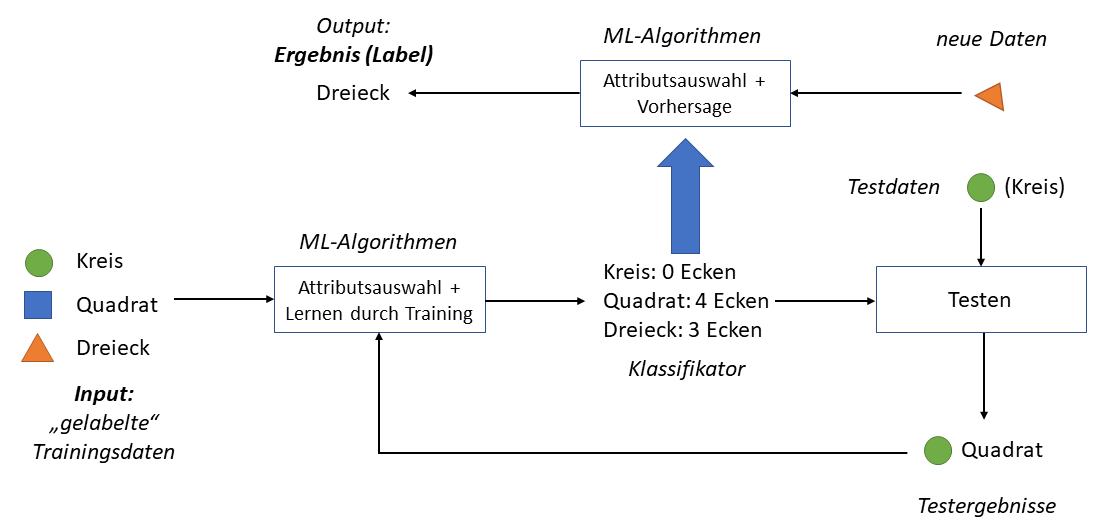
\includegraphics[width=\textwidth]{images/ML}
    \caption{Allgemeiner Prozess des überwachten Machine Learnings dargestellt anhand eines Beispiels (vereinfacht)}\label{fig:ml}
\end{figure}

Die Abbildung zeigt den Prozess des überwachten Machine Learnings anhand des Beispiels der Erlernung eines Klassifikators zur Erkennung beziehungsweise Vorhersage von geometrischen Formen. Der Prozess beginnt mit den \glqq gelabelten\grqq{} Eingabedaten (A). Die Werte der Label (kategorisch oder numerisch) stellen dabei die zu vorhersagende Zielklasse dar. In diesem Falle bilden die Namen der geometrischen Formen die Label als kategorischen Wert. Die Rohdaten der Eingabemenge bestehen aus den geometrischen Formen selbst. Beide Datenmengen bilden das Datenset. Um nun einen Klassifikator anlernen zu können, müssen Merkmale der Eingangsdaten ausgewählt werden, anhand derer diese identifiziert werden können (B). Diese zu identifizierenden Charakteristika der Daten werden Attribute genannt. Diese Attribute können bereits vor dem Erlernen festgelegt werden oder automatisiert extrahiert werden. Im vorliegenden Fall wurde die Anzahl der Ecken der geometrischen Formen als Attribut zur Erlernung ausgewählt. Das Ergebnis ist der fertig trainierte Klassifikator, welcher das erlernte Wissen auf neue Daten abbilden kann (C). Ein Teil des Datensets wird in der Regel verwendet, um den Klassifikator nach dessen Erstellung zu testen (D). Die in der Regel verwendeten Verhältnisse (englisch: Split-Ratio) zwischen Trainings- und Testdaten betragen 80:20 (basierend auf dem Paretoprinzip) oder 75:25 (zum Beispiel \cite{Queiroz2016}). Diese Testdaten werden dem Klassifikator als Eingabemenge zur Klassifikation ohne Label zur Verfügung gestellt. Die Label sollten jedoch nicht verworfen werden, da sie als Vergleichsgrundlage für die Verhersageperformanz des Klassifikators dienen. Sie bilden die sogenannte \glqq Ground Truth\grqq (deutsch: Grundwahrheit). Dazu werden die vom Klassifikator vorhergesagten Label mit denen der Ground Truth verglichen. Sollte dieser Vergleich ergeben, dass die Label große Abweichungen zeigen, so kann der Klassifikator erneut erlernt werden mit anderen Attributen oder einer veränderten Split-Ratio. Erfüllt der Klassifikator die Anforderungen an die Performanz der Vorhersagen, so ist dieser bereit Vorhersagen auf Basis neuer Eingabedaten zu treffen (E). Dazu müssen von den neuen Daten die Attribute ermittelt werden. Auf Basis dieser trifft der Klassifikator die Vorhersage und liefert als Ausgabe das Label des Wertes der Zielklasse.

Der in \autoref{fig:ml} dargestellte Klassifikator stellt einen multinomiellen oder multi-class Klassifikator dar, da er zu drei oder mehr Werten der Zielklasse zuordnen kann \cite{Sammut2017}. Für viele praktische Anwendungen genügt jedoch ein binärer Klassifikator, welcher Vorhersagen zu zwei Werten der Zielklasse trifft. Dies trifft auch auf die Klassifikatoren dieser Arbeit zu.

\section{Fehlervorhersage mittels Machine Learning}

Der Hintergrund zur Fehlervorhersage mittels Machine Learning wird anhand eines Beispiels aus der Literatur erläutert. Es stammt aus einer wissenschaftlichen Arbeit von Queiroz et al. \cite{Queiroz2016} und widmet sich der Fehlervorsage von Features. Bei dieser ersten Fallstudie handelt es sich um die bisher einzige Arbeit mit Bezug zu Software-Features und stellt somit für diese Masterarbeit eine bedeutende literarische Grundlage dar. Der Ablauf des von Queiroz et al. angewandten Prozesses zur Erstellung eines featurebasierten Datensets und dessen Anwendung zur Erlernung von Klassifikatoren orientiert sich am zuvor vorgestellten allgemeinen Prozess des überwachten Machine Learnings.

Die Erläuterung des Beispiels erfolgt anhand von zwei Abbildungen, welche den in der Arbeit von Queiroz et al. vorgestellten Prozess in zwei Teilen visualisieren. Der erste Teil ist in \autoref{fig:ml1} dargestellt.

\begin{figure}[H]
    \centering
    \captionsetup{justification=centering}
    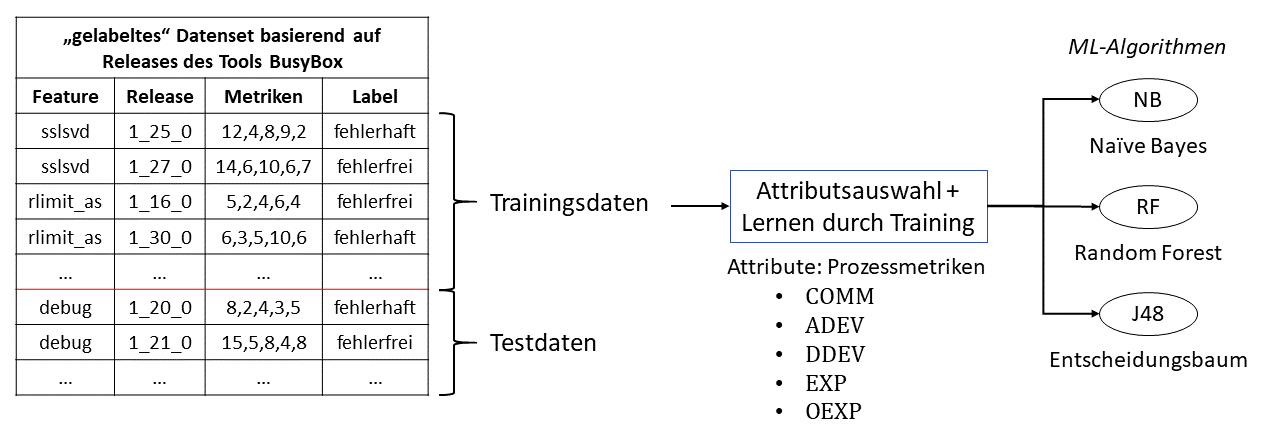
\includegraphics[width=\textwidth]{images/ML1}
    \caption{Teil 1: Featurebasierter Prozess des überwachten Machine Learnings nach \cite{Queiroz2016}}\label{fig:ml1}
\end{figure}

\subsection*{Datensatz}

Die Datenbasis des Datensets bilden historische Commits des UNIX-Toolkits BusyBox\footnote{\url{https://busybox.net/}}, dessen Quellcode frei verfügbar in einem Git-Repository\footnote{\url{https://git.busybox.net/busybox/}} eingesehen und von dort geklont werden kann. Diese Commits wurden wiederum ihren entsprechenden Releases zugeordnet, welche auf der vergebenen Tag-Struktur des Repositories beruhen. Ferner wurden aus den Diffs der Commits die dort bearbeiteten Features extrahiert und anschließend zusammen mit den Release-Informationen in einer MySQL-Datenbank gespeichert. Zusätzlich enthält jeder Datenbankeintrag aggregierte Werte von fünf auf das Feature und den Release bezogenen Prozessmetriken (Erläuterung folgt) sowie das binäre Label, ob ein Feature in einem Release fehlerhaft oder fehlerfrei war. Ein Feature gilt in einem Release als fehlerhaft, sofern in einem Commit des darauffolgenden Releases ein fehlerbehebender Commit bezüglich des Features festgestellt werden konnte. Dies geschieht über die Analyse der Commit-Nachrichten. Sofern eine Commit-Nachricht die Begriffe \glqq bug\grqq{} (Fehler), \glqq error\grqq{} (schwerwiegender Fehler), \glqq fail\grqq{} (fehlschlagen) oder \glqq fix\grqq{} (beheben) enthält, werten die Autoren des Papers den Commit als fehlerbehebend. Alternative Methoden zur Durchführung dieser Analyse bestehen aus der Eindbindung von Daten aus Bug-Tracking-Systemen, die häufig an Software-Repositories angebunden sind, sowie aus der Anwendung des sogenannten SZZ-Algorithmus, welcher in dieser Arbeit verwendet wurde und in \hyperref[szz-def]{Abschnitt 3.2} erläutert wird \cite{Sliwerski2005,Zimmermann2007}. Wie im Rahmen des überwachten Machine Learning üblich, wird das Datenset in Trainings- und Testdaten in einem Verhältnis von 75:25 geteilt. 

\subsection*{Metriken und Klassifikation}

Die Trainingsdaten werden dann den Klassifikatoren zur Erlernung zur Verfügung gestellt. Als Attribute dienen fünf Prozessmetriken mit spezifischer Betrachtung von Software-Features. Einen Überblick über die Beschreibungen dieser gibt \autoref{tab:metrics-rodrigo}. Als Klassifikationsalgorithmen wurden Na\"{\i}ve Bayes, Random Forest und J48-Entscheidungsbäume gewählt. Diese Algorithmen wurden unter anderem auch in dieser Arbeit verwendet. Erläuterungen können in \hyperref[algorithms]{Abschnitt 4.1} gefunden werden.

\begin{table}[t]
\centering
\caption{Übersicht der von \cite{Queiroz2016} verwendeten Prozessmetriken}
\label{tab:metrics-rodrigo}
\begin{tabular}{|c|l|} 
\hline
\textbf{Metrik}  & \textbf{Beschreibung}  \\ 
\hline
COMM & \begin{tabular}[c]{@{}l@{}}Anzahl der Commits, die in einem Release dem betreffenden \\ Feature gewidmet sind. \end{tabular} \\ 
\hline
ADEV & \begin{tabular}[c]{@{}l@{}}Anzahl der Entwickler, die das betreffende Feature\\in einem Release bearbeitet haben. \end{tabular} \\ 
\hline
DDEV & \begin{tabular}[c]{@{}l@{}}kummulierte Anzahl der Entwickler, die das betreffende Feature\\in einem Release bearbeitet haben. \end{tabular} \\ 
\hline
EXP & \begin{tabular}[c]{@{}l@{}}Geometrisches Mittel der \glqq Erfahrung\grqq{} aller Entwickler, die am \\ betreffenden Feature in einem Release gearbeitet haben. \end{tabular} \\ 
\hline
OEXP & \begin{tabular}[c]{@{}l@{}}\glqq Erfahrung\grqq{} des Entwicklers, der am meisten zum betreffenden \\ Feature in einem Release beigetragen hat. \end{tabular} \\ 
\hline
\multicolumn{2}{|c|}{\begin{tabular}[c]{@{}c@{}}Erfahrung ist definiert als Summe der geänderten, gelöschten\\oder hinzugefügten Zeilen im zugehörigen Release. \end{tabular}} \\
\hline
\end{tabular}
\end{table}

\begin{figure}[H]
    \centering
    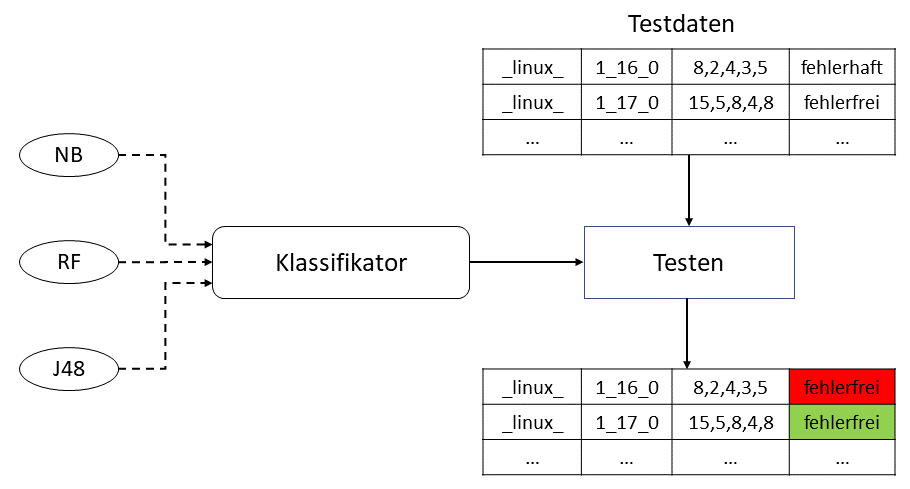
\includegraphics[width=0.8\textwidth]{images/ML2}
    \caption{Teil 2: Featurebasierter Prozess des überwachten Machine Learnings nach \cite{Queiroz2016}}\label{fig:ml2}
\end{figure}

\subsection*{Test der Klassifikatoren}

Wie in \autoref{fig:ml2} dargestellt ist, wird für jeden Klassifikationsalgorithmus ein Klassifikator erstellt, welcher anschließend getestet und evaluiert wird. Dazu werden die jeweiligen Klassifikatoren auf das Testdatenset angewendet, ohne jedoch die Werte der Zielklassen mit anzugeben. Diese werden im Anschluss an den Klassifikationsvorgang mit den vorhergesagten Werten auf Übereinstimmung verglichen. Anhand dieses Vergleiches können die Genauigkeit sowie weitere Metriken zur Bewertung der Leistung der Klassifikatoren gemessen werden. Eine Übersicht von Evaluationsmetriken kann in \hyperref[eval-metrics]{Abschnitt 5.2.1} gefunden werden.

Die so erstellten Klassifikatoren können dann zur Vorhersage von neuen Daten genutzt werden. Dazu müssen die fünf zuvor genannten Prozessmetriken der neuen Daten berechnet werden. 

\cleardoublepage
